\documentclass[10.5pt,a4paper,UTF8]{article}
\usepackage{geometry}
\geometry{margin=1in}
\usepackage{booktabs}
\usepackage{minted}
\usepackage{xcolor}
\usepackage{graphicx}
\usepackage{enumitem}
\usepackage{hyperref}
\usepackage{fontspec}
\usepackage{ctex}

\setmonofont{JetBrainsMono-Regular.ttf}[ItalicFont=JetBrainsMono-Italic.ttf,Path=C:/Users/31515/AppData/Local/Microsoft/Windows/Fonts/]
\setminted{breaklines=true, breakanywhere=true, style=colorful, fontsize=\fontsize{9pt}{11}, linenos=true}

\title{计算机网络实验1\\利用流式套接字编写聊天程序}
\author{鲁昕宁 2414015}
\date{\today}

\begin{document}
\begin{titlepage}
\maketitle
\end{titlepage}

\section{实验目的}
用 C++ 和 Winsock 基本套接字实现一个多人聊天程序，服务端与客户端都是 WinUI 3 窗口。实验要完成四件事：
\begin{enumerate}[leftmargin=2em]
    \item 为 TCP 字节流设计带长度的应用层帧，使一条消息不会被粘在一起或从中间拆开；
    \item 用多线程同时服务多个客户，界面线程只负责显示；
    \item 支持英文和中文；
    \item 用每条帧上的序号观察连接存活时有没有丢消息。
\end{enumerate}

\section{实验环境}
程序使用 C++17。套接字只调用 Winsock2 的 \texttt{socket}、\texttt{bind}、\texttt{listen}、\texttt{accept}、\texttt{connect}、\texttt{send}、\texttt{recv} 和 \texttt{closesocket}。每个客户连接由一个 \texttt{std::thread} 接收，界面更新通过 WinUI 的 \texttt{DispatcherQueue.TryEnqueue} 回到 UI 线程。

编译环境为 Visual Studio 2022 Professional，平台工具集 v143，Windows SDK \texttt{10.0.22621.0}，Windows App SDK 1.6。工程是自包含运行库的桌面程序。可执行文件放在 \texttt{bin} 目录下，分别是服务端和客户端。

\section{聊天协议}
TCP 交给应用的是字节流。一次 \texttt{recv} 可能只得到半条消息，也可能一次得到多条。协议因此使用固定 10 字节头加 UTF-8 负载。多字节整数使用网络字节序。负载最长 1024 字节。

\begin{table}[htbp]
\centering
\caption{帧头布局}
\label{tab:header}
\begin{tabular}{lll}
\toprule
偏移 & 长度 & 含义 \\
\midrule
0 & 2 & 魔数 \texttt{0x43 0x48}（\texttt{CH}） \\
2 & 1 & 版本，当前为 1 \\
3 & 1 & 消息类型 \\
4 & 4 & 序号 \texttt{uint32}，每条连接的每个方向从 1 递增 \\
8 & 2 & 负载长度 \texttt{uint16} \\
10 & $n$ & UTF-8 负载 \\
\bottomrule
\end{tabular}
\end{table}

发送时循环调用 \texttt{send}，直到 10 字节头和全部负载都写完。接收时先读满 10 字节，校验魔数、版本和长度，再按长度读满负载。魔数、版本或长度非法时，服务端关闭该连接。

\begin{table}[htbp]
\centering
\caption{消息类型}
\label{tab:type}
\begin{tabular}{cll}
\toprule
值 & 名称 & 作用 \\
\midrule
1 & HELLO & 客户登记昵称 \\
2 & WELCOME & 服务端确认登记 \\
3 & CHAT & 聊天文本。转发时负载为“昵称: 正文” \\
4 & NOTICE & 加入、离开或在线列表 \\
5 & LIST & 客户请求在线列表 \\
6 & QUIT & 客户主动退出 \\
7 & ERR & 昵称、编码或长度不合法 \\
\bottomrule
\end{tabular}
\end{table}

昵称是 1 到 16 个 Unicode 字符，不允许控制字符。重名会被拒绝。默认端口是 9000。客户点“断开”或关闭窗口时先发 QUIT，再关闭套接字并等待接收线程结束。服务端点“停止”时停止 \texttt{accept}，关闭已有连接。\texttt{recv} 返回 0 或错误时，服务端从客户表删除该连接，并向其他人广播离开通知。

\section{程序结构}
\subsection{源码目录}
源码按“协议和套接字核心”与“窗口”分开。窗口工程只负责输入和显示，套接字调用集中在 \texttt{shared}。这样服务端窗口、客户端窗口和环回测试可以共用同一套组帧与收发代码。

\begin{minted}{text}
lab1/
  Chat.sln              解决方案：服务端、客户端、环回测试
  build.bat             调用 MSBuild 生成 Release x64
  shared/
    protocol.h          帧布局、消息类型、默认端口
    netutil.h/.cpp      组帧、拆帧、UTF-8 与 UTF-16 转换
    server_core.h/.cpp  监听、客户表、转发
    client_core.h/.cpp  连接、发送、接收、序号统计
  server/               WinUI 服务端窗口
    App.xaml.cpp        启动应用
    MainWindow.xaml.cpp 端口、在线用户、日志
  client/               WinUI 客户端窗口
    App.xaml.cpp        启动应用
    MainWindow.xaml.cpp 连接、消息列表、连续发送
  tests/
    loopback.cpp        不带界面的 100 条环回测试
  bin/                  编译得到的可执行文件和运行库
\end{minted}

\texttt{server} 与 \texttt{client} 各自是一个 WinUI 工程。\texttt{MainWindow.idl} 声明窗口运行时类，界面在 \texttt{MainWindow.xaml.cpp} 里用代码搭出来。\texttt{pch.h} 先包含 Winsock2，再包含 WinUI 头文件，避免 \texttt{windows.h} 抢先声明套接字类型。\texttt{tests/loopback.cpp} 直接调用 \texttt{ChatServer} 和 \texttt{ChatClient}，用来在没有窗口的情况下核对中文消息和序号。\texttt{bin} 是输出目录，其中的动态库是自包含运行库，和源码分开。

\subsection{组帧与拆帧}
\texttt{send} 和 \texttt{recv} 都不保证一次调用搬完调用者给出的全部字节。\texttt{send\_all} 和 \texttt{recv\_exact} 用循环把短发送、短接收补齐，失败或对端关闭时返回假。

\inputminted[firstline=106,lastline=128,linenos,firstnumber=106]{cpp}{shared/netutil.cpp}

\texttt{send\_frame} 按协议填写 10 字节头。序号和长度写成网络序，然后先后写出头部和负载。\texttt{recv\_frame} 先读满头部，再按头部中的长度读负载。魔数、版本、类型或长度不合法时返回协议错误，服务端随即关闭这条连接。粘在同一次 \texttt{recv} 里的多条消息，会在后面的循环中被拆开。只到达一半的消息会留在循环里，直到剩余字节到齐。

\inputminted[firstline=150,lastline=184,linenos,firstnumber=150]{cpp}{shared/netutil.cpp}

\subsection{服务端的客户线程与转发}
\texttt{accept\_loop} 每接受一个连接，就把客户放进客户表，并单独启动接收线程。客户表由互斥锁 \texttt{clients\_mu\_} 保护。每个客户另有发送锁 \texttt{send\_mu}。\texttt{send\_to} 持有这把锁之后才写套接字，因此两个线程不会同时写同一个连接。

CHAT 先检查 UTF-8，再在正文前加上发送者昵称，然后 \texttt{broadcast}。广播时先在锁内复制客户表，锁外再逐个发送，避免发送阻塞期间一直占着客户表。参数 \texttt{except} 是发送者本人，所以消息不会回显。连续发送只在第 1 条、最后一条和每 20 条写日志。

\inputminted[firstline=203,lastline=221,linenos,firstnumber=203]{cpp}{shared/server_core.cpp}

\inputminted[firstline=276,lastline=288,linenos,firstnumber=276]{cpp}{shared/server_core.cpp}

\subsection{客户端的序号检查与退出}
接收线程每得到一帧就调用 \texttt{note\_seq}。期望序号从 1 开始，收到的序号等于期望值时只把期望值加 1；否则把缺口累加到 \texttt{gaps}，并把下一次期望改成当前序号的下一个。状态栏根据 \texttt{seq\_ok} 显示“序号连续”或“序号空洞”。CHAT 负载里的 \texttt{burst i/n} 另外用一个标记数组统计测试条数，避免同一序号被重复计入。

\inputminted[firstline=260,lastline=274,linenos,firstnumber=260]{cpp}{shared/client_core.cpp}

断开时先在发送锁内发出 QUIT 并 \texttt{shutdown}，释放锁之后再 \texttt{join} 连续发送线程和接收线程，最后 \texttt{closesocket}。发送锁不能在 \texttt{join} 期间一直持有，否则接收线程若还要取这把锁就会死锁。

\subsection{界面线程}
套接字线程不接触控件。服务端的日志回调和在线名单回调、客户端的消息回调，都通过 \texttt{post} 把闭包排到 UI 线程。\texttt{open\_} 在窗口关闭时置假，避免关闭过程中再改已经销毁的控件。

\inputminted[firstline=165,lastline=178,linenos,firstnumber=165]{cpp}{client/MainWindow.xaml.cpp}

\section{界面与测试}
服务端窗口有端口、开始监听、停止、在线用户和日志，见图~\ref{fig:server}。客户端窗口有地址、端口、昵称、消息列表、输入框和连续发送，状态栏在最下方。

三名用户同时连到 \texttt{127.0.0.1:9000}：张三、Alice 和李四。张三发送 \texttt{Hello} 和“你好，晚上见”，Alice 回复 \texttt{Good evening 晚上好}。Alice 的窗口同时出现英文和中文，见图~\ref{fig:alice}。协议负载始终是 UTF-8 字节，WinUI 文本框本身使用 Unicode，中文不依赖控制台代码页。

\begin{figure}[htbp]
    \centering
    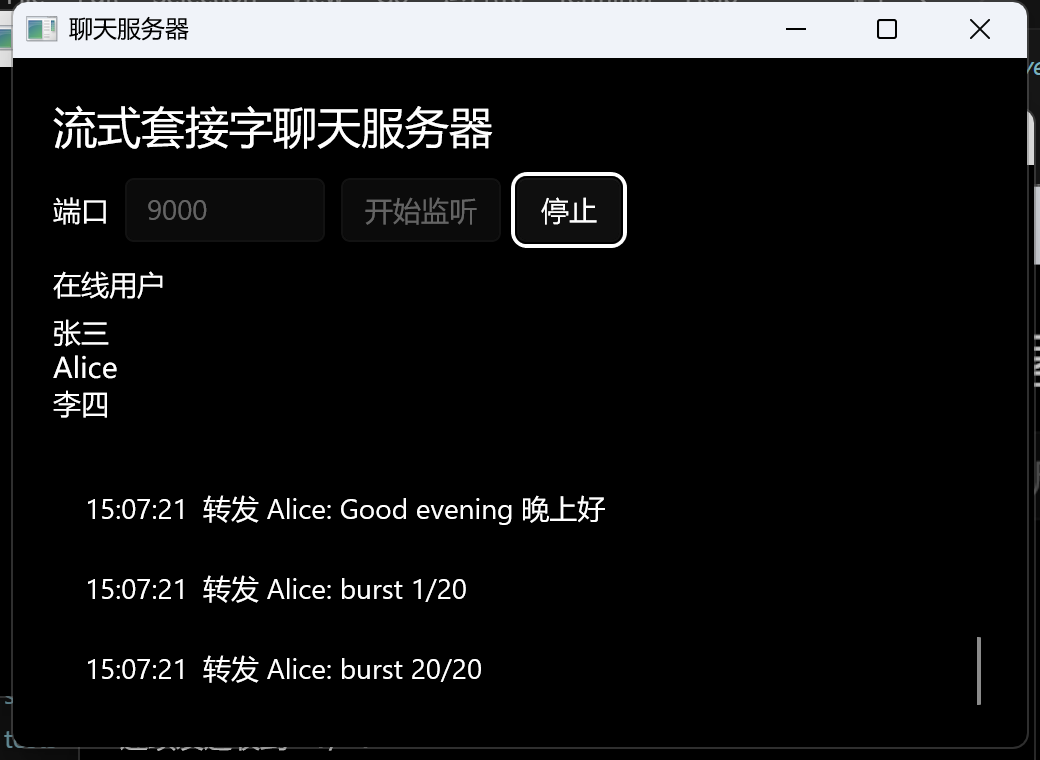
\includegraphics[width=0.72\textwidth]{figure/server.png}
    \caption{服务端正在监听 9000。在线用户为张三、Alice、李四，日志中有中文转发记录。}
    \label{fig:server}
\end{figure}

\begin{figure}[htbp]
    \centering
    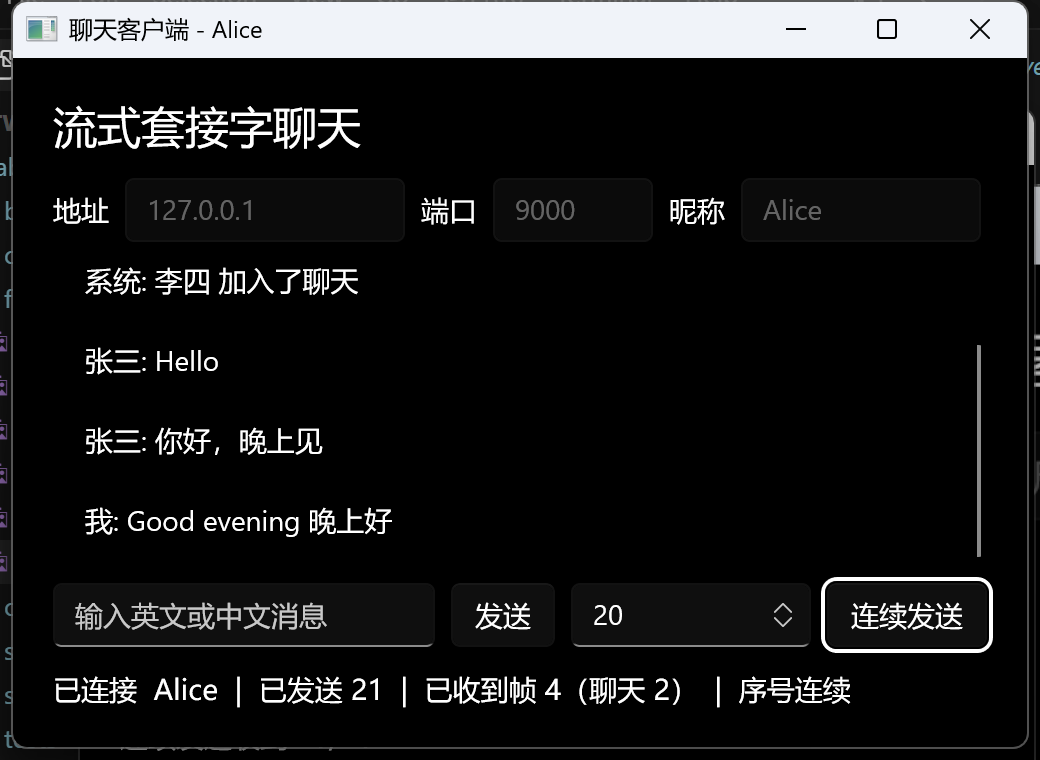
\includegraphics[width=0.72\textwidth]{figure/client-alice.png}
    \caption{Alice 收到张三的英文和中文，并发送了中英混合的回复。}
    \label{fig:alice}
\end{figure}

李四点击“在线列表”后，收到“在线用户：张三、Alice、李四”，见图~\ref{fig:li}。张三点“断开”之后，Alice 收到“张三 离开了聊天”，见图~\ref{fig:leave}。服务端在线名单随之去掉张三，并在日志中记下离开，见图~\ref{fig:server-leave}。

\begin{figure}[htbp]
    \centering
    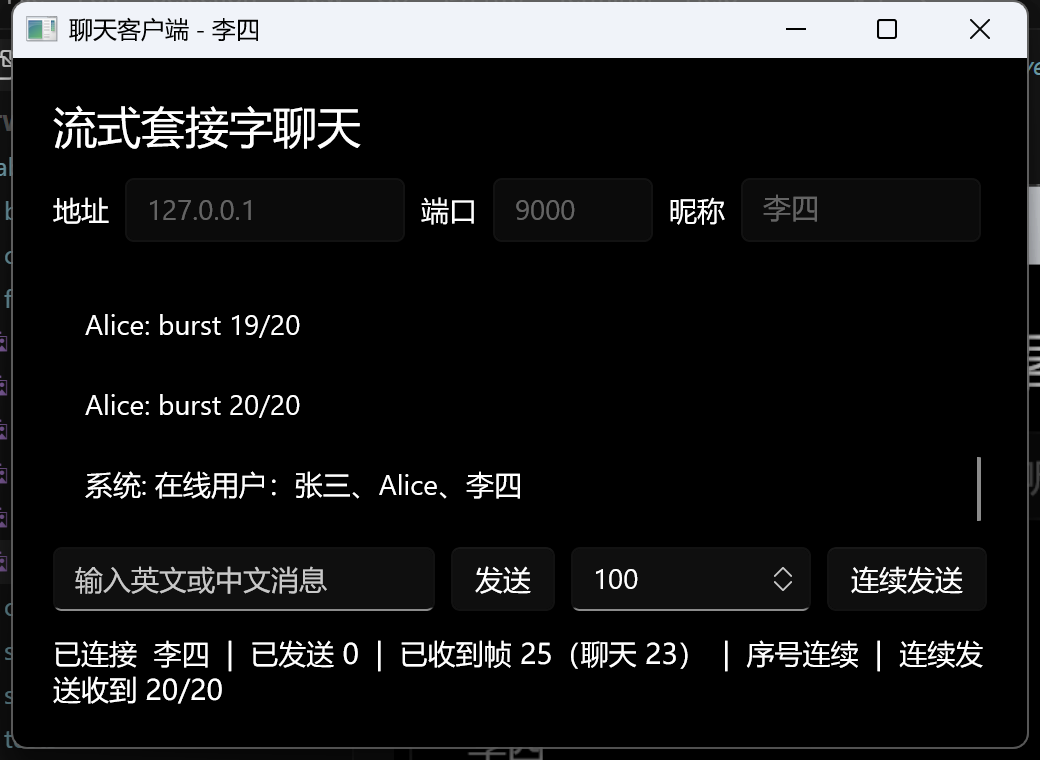
\includegraphics[width=0.72\textwidth]{figure/client-li.png}
    \caption{李四收到完整在线名单，状态栏显示序号连续，连续发送 20 条全部到达。}
    \label{fig:li}
\end{figure}

\begin{figure}[htbp]
    \centering
    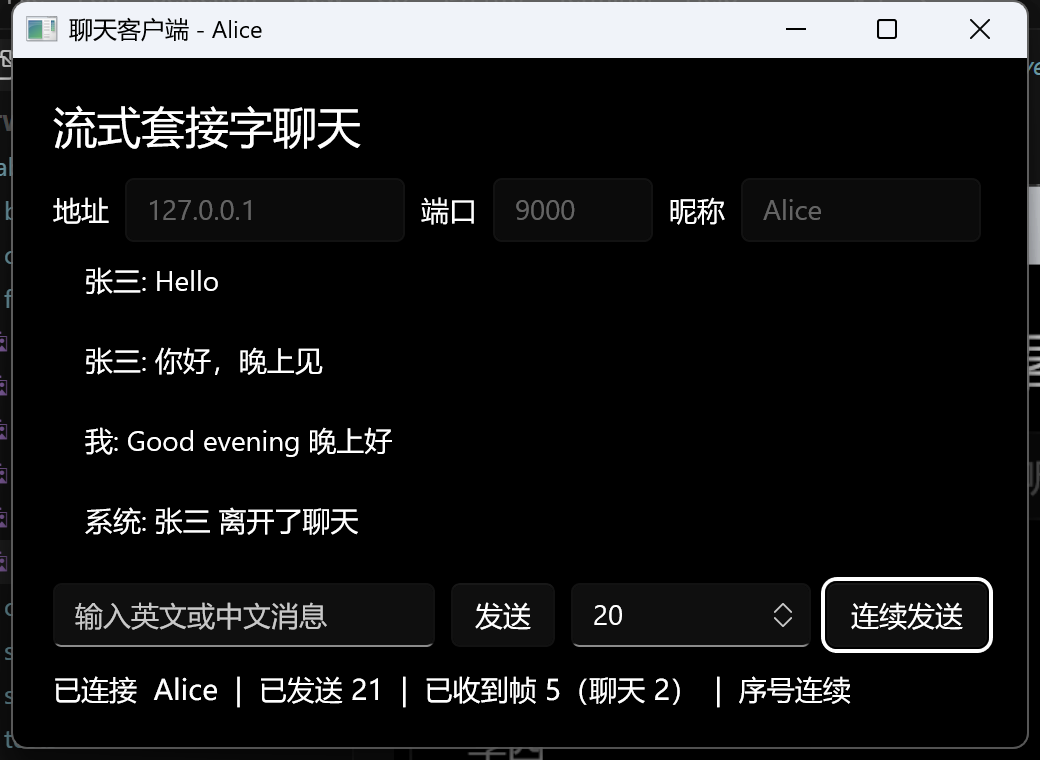
\includegraphics[width=0.72\textwidth]{figure/client-leave.png}
    \caption{张三断开后，Alice 收到离开通知。此前的英文和中文消息都还在。}
    \label{fig:leave}
\end{figure}

\begin{figure}[htbp]
    \centering
    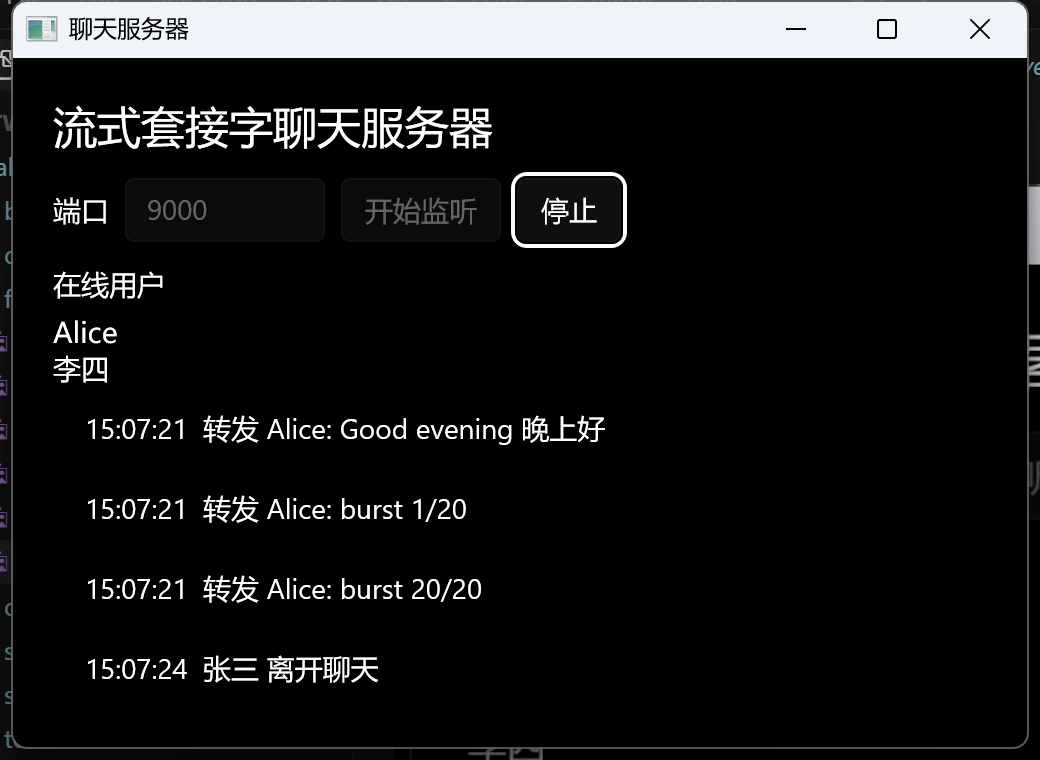
\includegraphics[width=0.72\textwidth]{figure/server-after-leave.png}
    \caption{张三离开后，在线用户剩下 Alice 和李四。}
    \label{fig:server-leave}
\end{figure}

\section{序号连续性}
序号属于某一条连接上的一个方向，从 1 开始，每成功组一帧加 1。接收方若发现新序号不是上一个序号加 1，就把该间隔计为序号空洞。

界面上的“连续发送”让 Alice 连续发出 20 条 \texttt{burst i/20}。张三的状态栏为：已发送 2，已收到帧 24（聊天 21），序号连续，连续发送收到 20/20，见图~\ref{fig:zhang}。20 条测试消息和它前面的聊天帧都按序号到齐。李四一侧同样是“序号连续”和“连续发送收到 20/20”。

另有一个不带界面的环回程序，在本机用同一套服务端和客户端核心发送 100 条。运行结果为：

\begin{minted}{text}
英文消息: Hello
中文消息: 你好，晚上见 / Good evening 晚上好
在线用户包含张三、Alice、李四
未连接  |  已发送 1  |  已收到帧 105（聊天 102）  |  序号连续  |  连续发送收到 100/100
序号空洞: 0
PASS
\end{minted}

\begin{figure}[htbp]
    \centering
    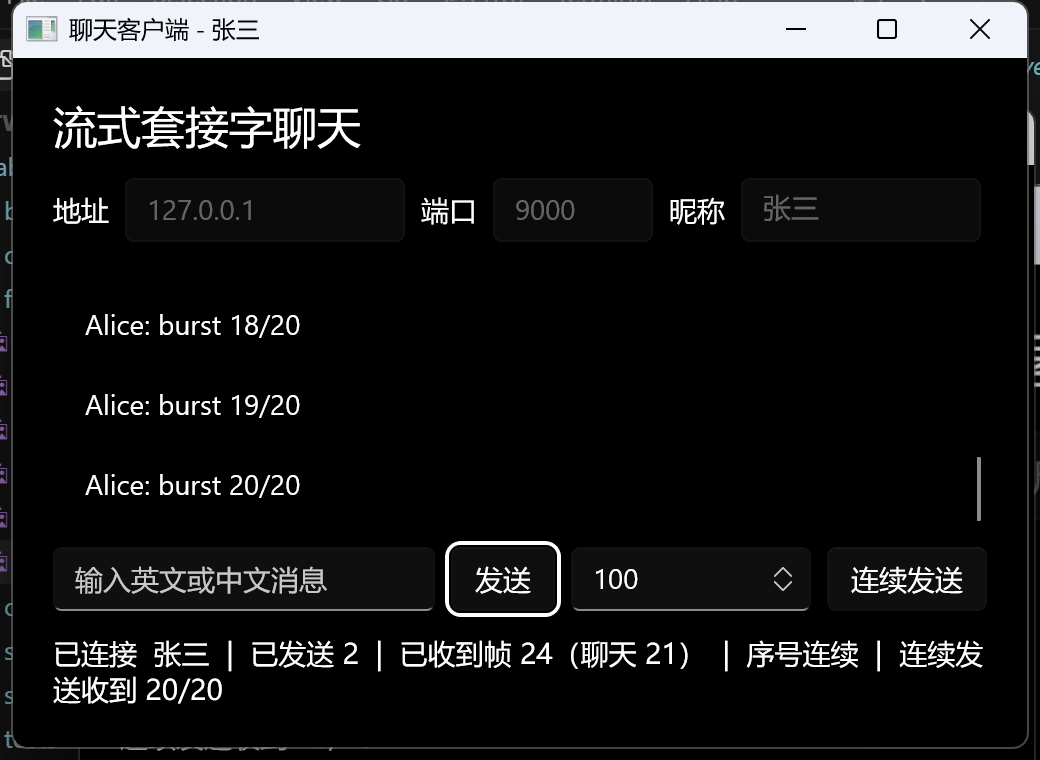
\includegraphics[width=0.72\textwidth]{figure/client-zhang.png}
    \caption{张三收到 Alice 的连续发送。状态栏显示序号连续，20 条全部到达。}
    \label{fig:zhang}
\end{figure}

TCP 会重传丢失的报文段。连接一直活着时，应用层读到的字节流是完整的，所以帧序号保持连续。若去掉长度字段，同一次 \texttt{recv} 可能把两条消息粘在一起，或者只拿到一条消息的前半段，看起来像内容损坏。那是字节流的分段，序号空洞并不会因此出现。

连接被强行掐断时，还没进入对端接收缓冲的数据会随这条连接消失。接收方看到的是 \texttt{recv} 返回 0 或错误，然后连接结束。这和链路上随机丢掉一个报文段不同：后者由 TCP 重传补上，前者是连接本身被取消了。

\section{结论}
实验用固定长度帧把 TCP 字节流还原成一条条聊天消息，并用每个方向独立递增的序号检查有没有缺帧。英文、中文和三人同时在线都工作正常。界面连续发送 20 条、环回测试连续发送 100 条时，接收方的序号都没有空洞，收到的测试条数与发送条数一致。连接存活期间，应用层观察不到消息的丢失。
\end{document}
